\documentclass[export]{beamer}

\usepackage[utf8]{inputenc}
\usepackage[T1]{fontenc}
    
\usepackage{standalone}
    
\usepackage[acronym]{glossaries}
    
\usepackage{enumitem}
    
\usepackage{xcolor}
    
\usepackage{multirow}
\usepackage{multicol}
    
\usepackage{array}
\newcolumntype{x}[1]{>{\centering\let\newline\\\arraybackslash\hspace{0pt}}p{#1}}
\usepackage{booktabs}
    
\usepackage{siunitx}
\usepackage{mathrsfs, amsmath}
    
\usepackage{graphicx}
\usepackage[font={small, color=IGNDarkGrey}, labelformat=empty]{caption}
\usepackage{subcaption}
\DeclareCaptionFont{tiny}{\tiny}
% \captionsetup[subtable]{labelfont={tiny, bf},textfont=normalfont,justification=raggedright}
\captionsetup[subfigure]{labelfont={tiny, bf},textfont=tiny,justification=raggedright}
\usepackage{adjustbox}

\usepackage{pifont}
\newcommand{\cmark}{{\color{green} \ding{51}}}%
\newcommand{\xmark}{{\color{red} \ding{55}}}%
    
\usepackage{hyperref}
    
\usepackage[
        mcite,
        backend=bibtex,
        style=verbose,
        citestyle=authoryear,
        bibstyle=numeric,
        sorting=none,
        autocite=footnote,
        maxnames=2,
        hyperref=true,
        natbib=true,
        abbreviate=true
    ]{biblatex}
\bibliography{references}
\setbeamerfont{footnote}{size=\tiny}


\usetheme{ign}


\newacronym{acr::lod}{LoD}{Level of Detail}
\newacronym{acr::elod}{eLoD}{evalution Level of Detail}
\newacronym{acr::lidar}{LiDAR}{Light Detection and Ranging}
\newacronym{acr::dsm}{DSM}{Digital Surface Model}
\newacronym{acr::gui}{GUI}{Graphical User Interface}

\title{Semantic 3D building model evaluation}
\subtitle{}
\institute[LaSTIG STRUDEL]{Univ. Paris Est, LaSTIG STRUDEL, IGN, ENSG}
\date{\today}
\author[O.Ennafii]{Oussama Ennafii}


\begin{document}

    \begin{frame}[plain]
        \titlepage{}
    \end{frame}

    \section{Introduction}
        \subsection{Context}
            \begin{frame}{3D model vs. 3D mesh}
                \begin{itemize}[label=$\blacktriangleright$, font=\color{IGNGreen}]
                    \item<1-> $3D$ urban model $\equiv$ polyhedral surface representing a building;
                    \item<2-> Each facet in a $3D$ model is akin to an architechtural feature;
                \end{itemize}
                \uncover<3>{
                    \begin{figure}
                        \includestandalone[mode=buildnew, width=\textwidth]{lods}
                    \end{figure}
                }
            \end{frame}
            \begin{frame}{Urban modeling}
                Modeling urban scenes, on a large scale, using sensor data:
                \begin{itemize}[label=$\blacktriangleright$, font=\color{IGNGreen}]
                    \item \acrfull{acr::lidar};
                    \item Stereoscopic images.
                \end{itemize}
            \end{frame}
        \subsection{Motivation}
            \begin{frame}{The need for modeling evaluation}
                \begin{itemize}[label=$\blacktriangleright$, font=\color{IGNGreen}]
                    \item<1-> Automatic urban modeling is an active research area~\citep{Musialski2012}, but not \textcolor{IGNRed}{yet operational}~\citep{rottensteiner2014results}:
                    \begin{itemize}[label=--]
                        \item reconstruction methods lack generality and compacity;
                        \item too many modelling errors require labourious manual corrections.
                    \end{itemize}
                    \item<2-> Urban $3D$ model semantic diagnostic is not well studied~\citep{nguatem2017modeling}.
                \end{itemize}
                ~\\
                \uncover<3->{
                    \begin{itemize}[label=Goal $\longrightarrow$, font=\color{purple}, leftmargin=2cm]
                        \item Detect and describe semantic errors that affects building $3D$ models.
                    \end{itemize}
                }
            \end{frame}
            \begin{frame}{Potential use}
                \begin{itemize}[label=$\blacktriangleright$, font=\color{IGNGreen}, itemsep=2em]
                    \item<1-> Change detection;
                    \item<2-> Urban models correction;
                    \item<3-> Urban reconstruction method evaluation;
                    \item<4-> Crowd reconstruction quality assessment.
                \end{itemize}
            \end{frame}
        \subsection{State of the art}
            \begin{frame}{How to classify quality evaluation methods?}
                \begin{itemize}[
                        label=$\blacktriangleright$,
                        font=\color{IGNGreen},
                        itemsep=2em
                    ]
                    \item<1-> Based on the output:
                    \begin{itemize}[label=--, itemsep=1em]
                        \item<2-> Geometric precision metrics;
                        \item<2-> Semantic errors.
                    \end{itemize}
                    \item<3-> Based on the reference data:
                    \begin{itemize}[label=--, itemsep=1em]
                        \item<4-> Manually obtained data;
                        \item<4-> Sensor data.
                    \end{itemize}
                \end{itemize}
            \end{frame}
            \begin{frame}[plain]{State-of-the-art summary}
                \begin{figure}
                    \includegraphics[width=\textwidth]{state_of_the_art}
                \end{figure}
            \end{frame}
            \begin{frame}{What do we want?}
                \begin{itemize}[label=$\blacktriangleright$, font=\color{IGNGreen}, itemsep=2em]
                    \item<1-> No reference data, or at least the most available sensor data;
                    \item<2-> Semantic errors independent from \textbf{reconstruction methods} and \textbf{urban scenes}.
                    \item<3-> Transferablility, and hence scallability, of the evalution method.
                \end{itemize}
            \end{frame}

    \section{Methodology}
        \begin{frame}{The evalutation pipeline sketch}
            \begin{figure}
                \includegraphics[width=\textwidth]{graphical_abstract}
            \end{figure}
        \end{frame}

        \subsection{Error taxonomy}
            \begin{frame}{Bidimensional taxonomy}
                In order to establish our taxonomy, two criterea are taken into account:
                \begin{itemize}[label=$\blacktriangleright$, font=\color{IGNGreen}]
                    \item<1-> the \acrshort{acr::lod};
                    \item<2-> the \emph{finesse}: the semantization evaluation level.
                    \begin{itemize}
                        \item<3-> an error is of maximal \emph{finesse} $\Rightarrow$ corresponds to a unit (semantically) action required for the operator to correct the model: $\equiv$ \emph{atomic} error.
                    \end{itemize}
                \end{itemize}
            \end{frame}
            \begin{frame}{Taxonomy \emph{finesse}}
                \begin{enumerate}[label = (\roman*)., font=\color{IGNGreen}]
                    \item<1-> \emph{finesse} $= 0$ $\longrightarrow$ \textbf{Unqualifiable} / \textbf{Qualifiable};
                    \item<2-> \emph{finesse} $= 1$ $\longrightarrow$ \textbf{Valid} / \textbf{Erroneous};
                    \item<3-> \emph{finesse} $= 2$:
                    \begin{itemize}[leftmargin=12em, font=\color{IGNDarkOrange}]
                        \item[\acrshort{acr::lod}-0 $\cup$ \acrshort{acr::lod}-1 $\longrightarrow$] \textbf{Building Errors}
                        \item[\acrshort{acr::lod}-2 $\longrightarrow$] \textbf{Facet Errors}
                        \item[\acrshort{acr::lod}-3 $\longrightarrow$] \textbf{Superstructure Errors}
                    \end{itemize}
                    \begin{figure}[H]
                        \begin{center}
                            \includestandalone[height=.2\textheight]{lods}
                        \end{center}
                    \end{figure}
                    \item<4-> \emph{finesse} $= 3$ $\longrightarrow$ \emph{atomic} errors.
                \end{enumerate}
            \end{frame}
            \begin{frame}[plain]{\emph{Atomic} errors for $2.5D$ overhead reconstruction}
                \only<1>{
                    \begin{figure}
                        \begin{center}
                            \begin{subfigure}{.28\textwidth}
                                \fbox{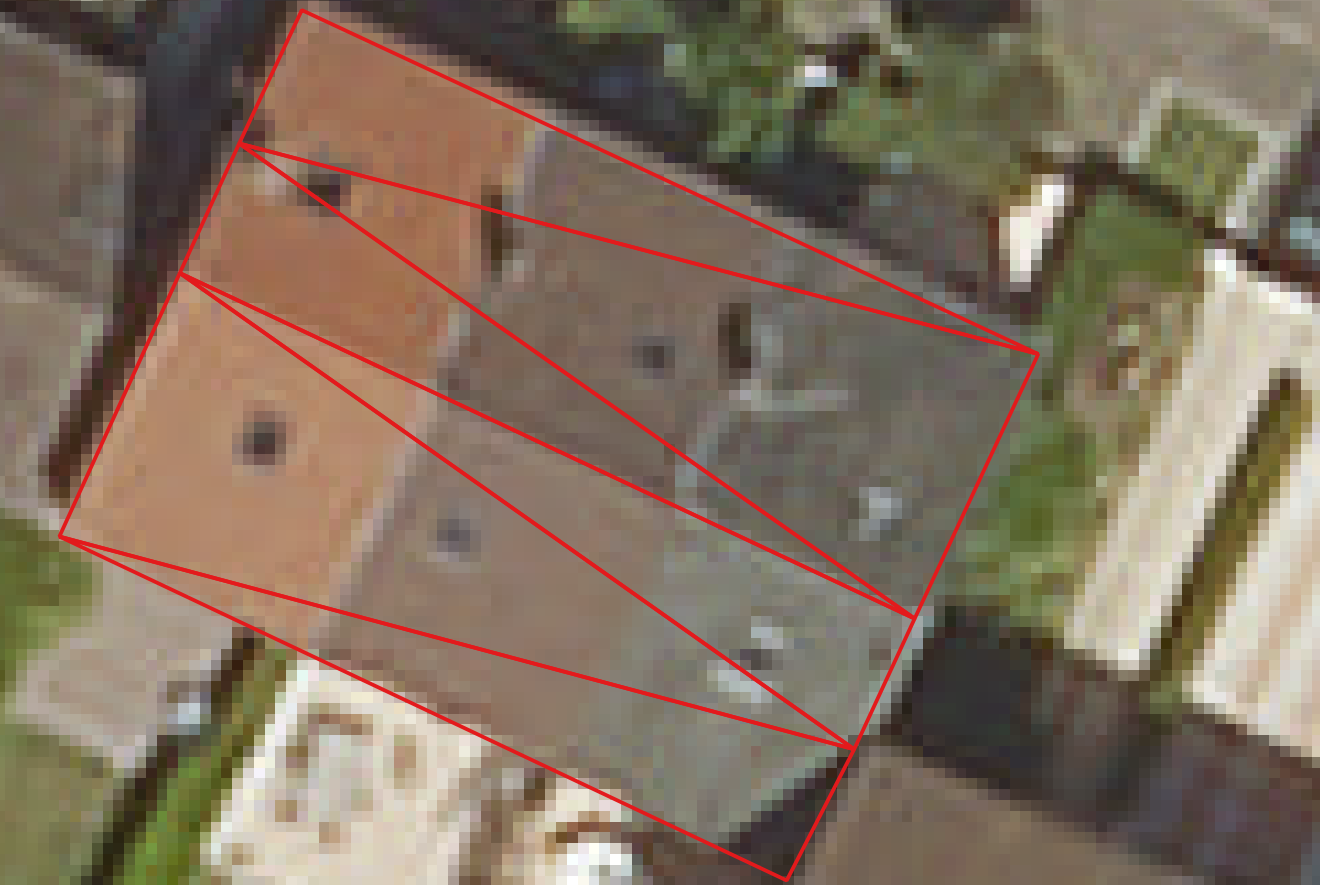
\includegraphics[width=\textwidth]{images/errors/building/under_segmentation}}
                                \caption{\label{fig::bul_under} Building under segmentation}
                            \end{subfigure}
                            \hspace{10pt}
                            \begin{subfigure}{.28\textwidth}
                                \fbox{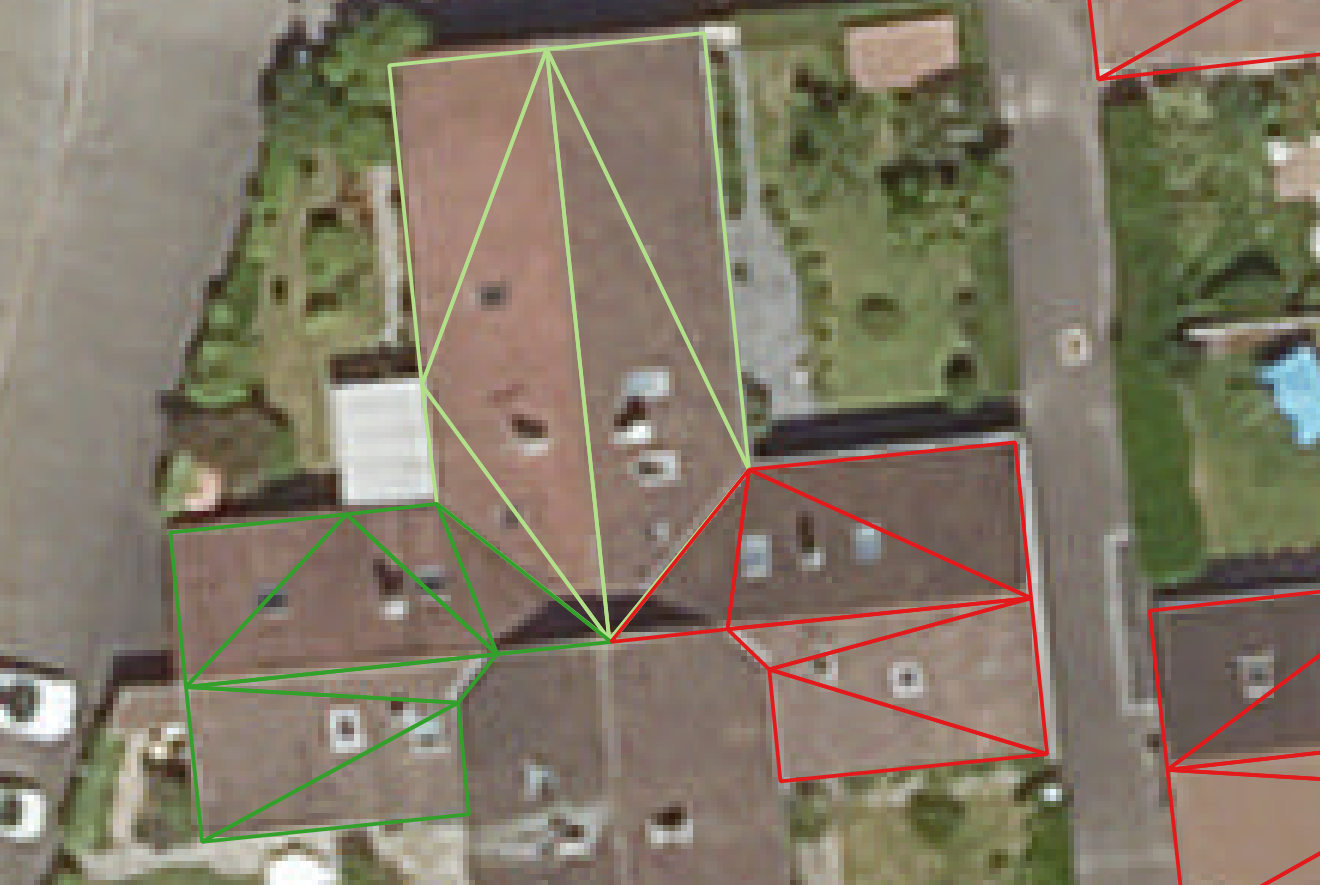
\includegraphics[width=\textwidth]{images/errors/building/over_segmentation}}
                                \caption{\label{fig::bul_over} Building over segmentation}
                            \end{subfigure}
                            \hspace{10pt}
                            \begin{subfigure}{.28\textwidth}
                                \fbox{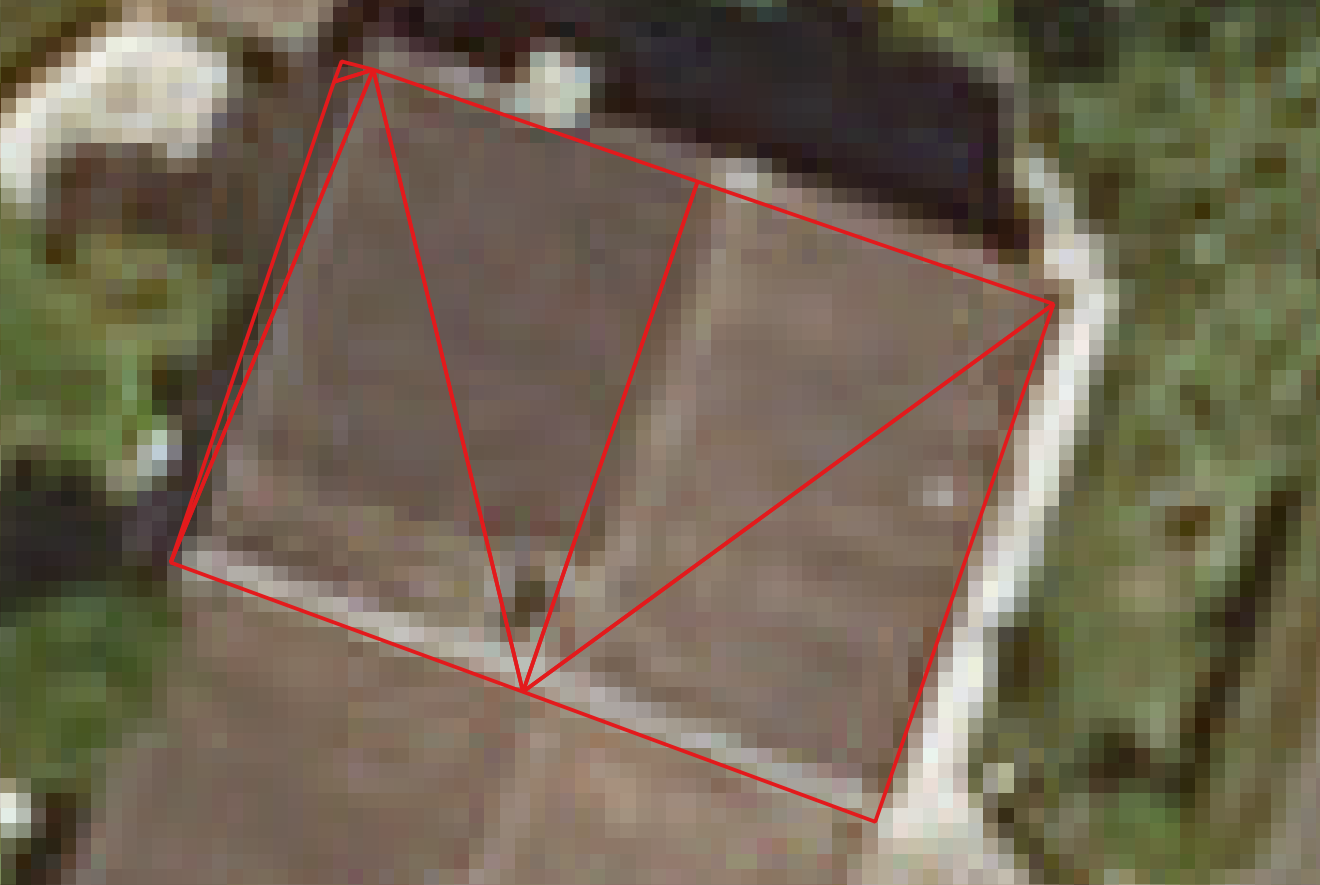
\includegraphics[width=\textwidth]{images/errors/building/footprint}}
                                \caption{\label{fig::bul_footprint} Imprecise footprint border}
                            \end{subfigure}
                            \hspace{10pt}
                            \begin{subfigure}{.28\textwidth}
                                \fbox{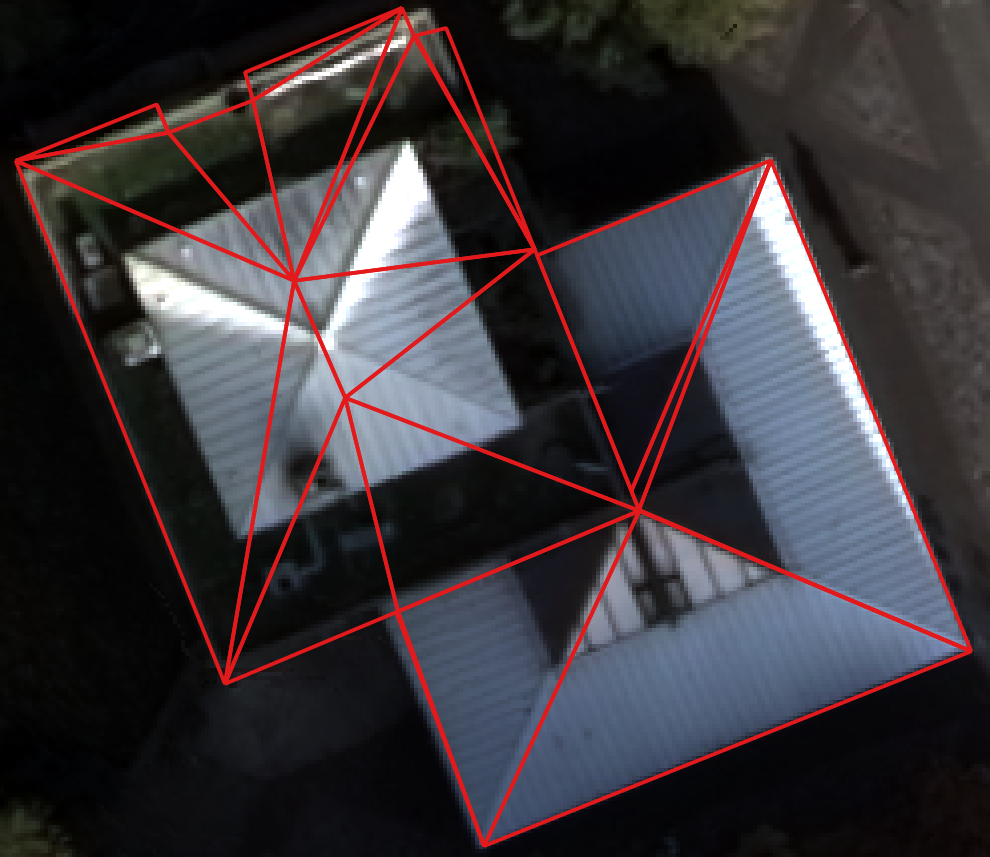
\includegraphics[width=\textwidth]{images/errors/building/footprint_topology}}
                                \caption{\label{fig::bul_height} Inaccurate footprint topology}
                            \end{subfigure}
                            \caption{Building \emph{atomic} errors illustration.}
                        \end{center}
                    \end{figure}
                }
                \only<2>{
                    \begin{figure}
                        \begin{center}
                            \begin{subfigure}{.28\textwidth}
                                \fbox{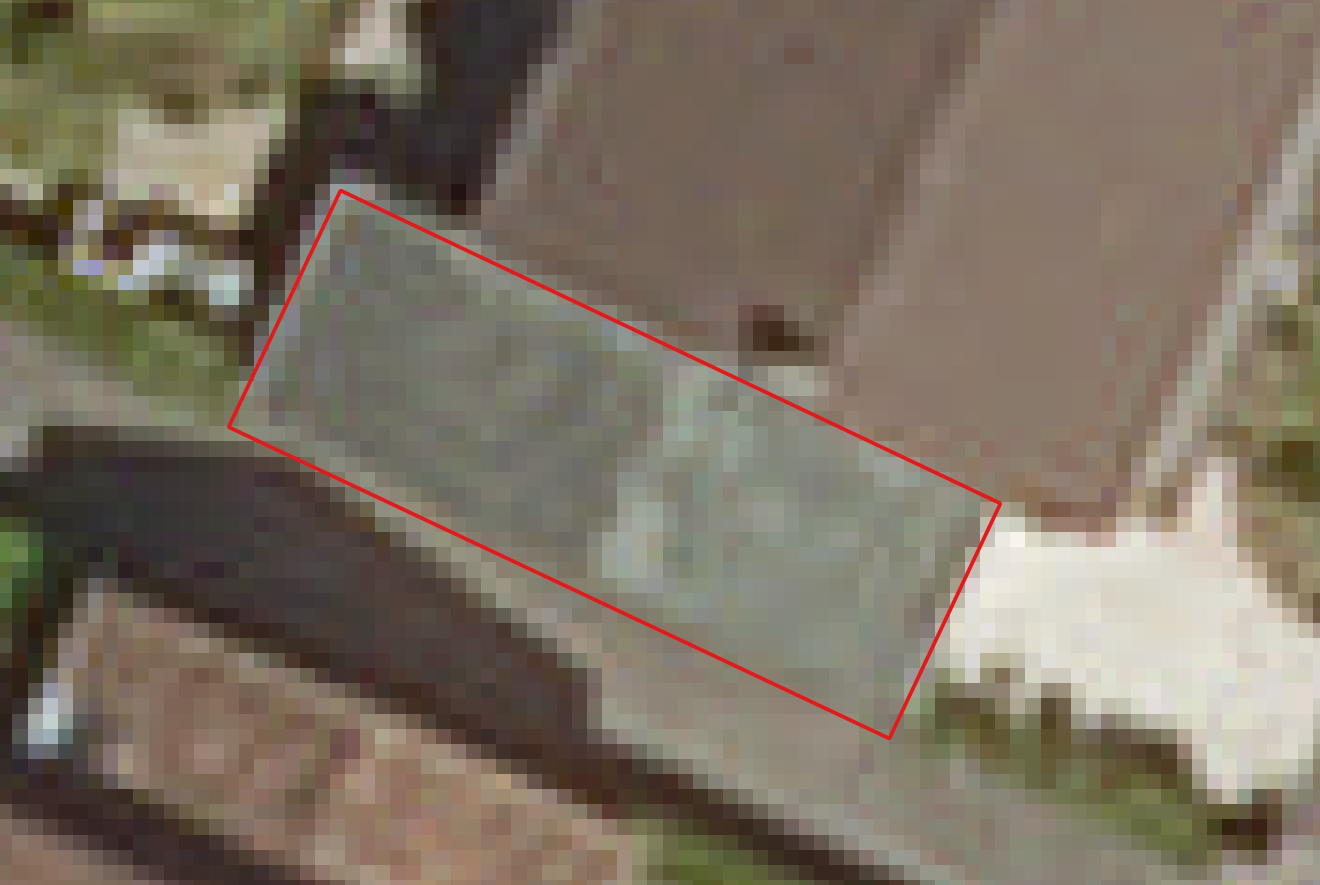
\includegraphics[width=\textwidth]{images/errors/facet/under_segmentation}}
                                \caption{\label{fig::fac_under} Facet under segmentation}
                            \end{subfigure}
                            \hspace{10pt}
                            \begin{subfigure}{.28\textwidth}
                                \fbox{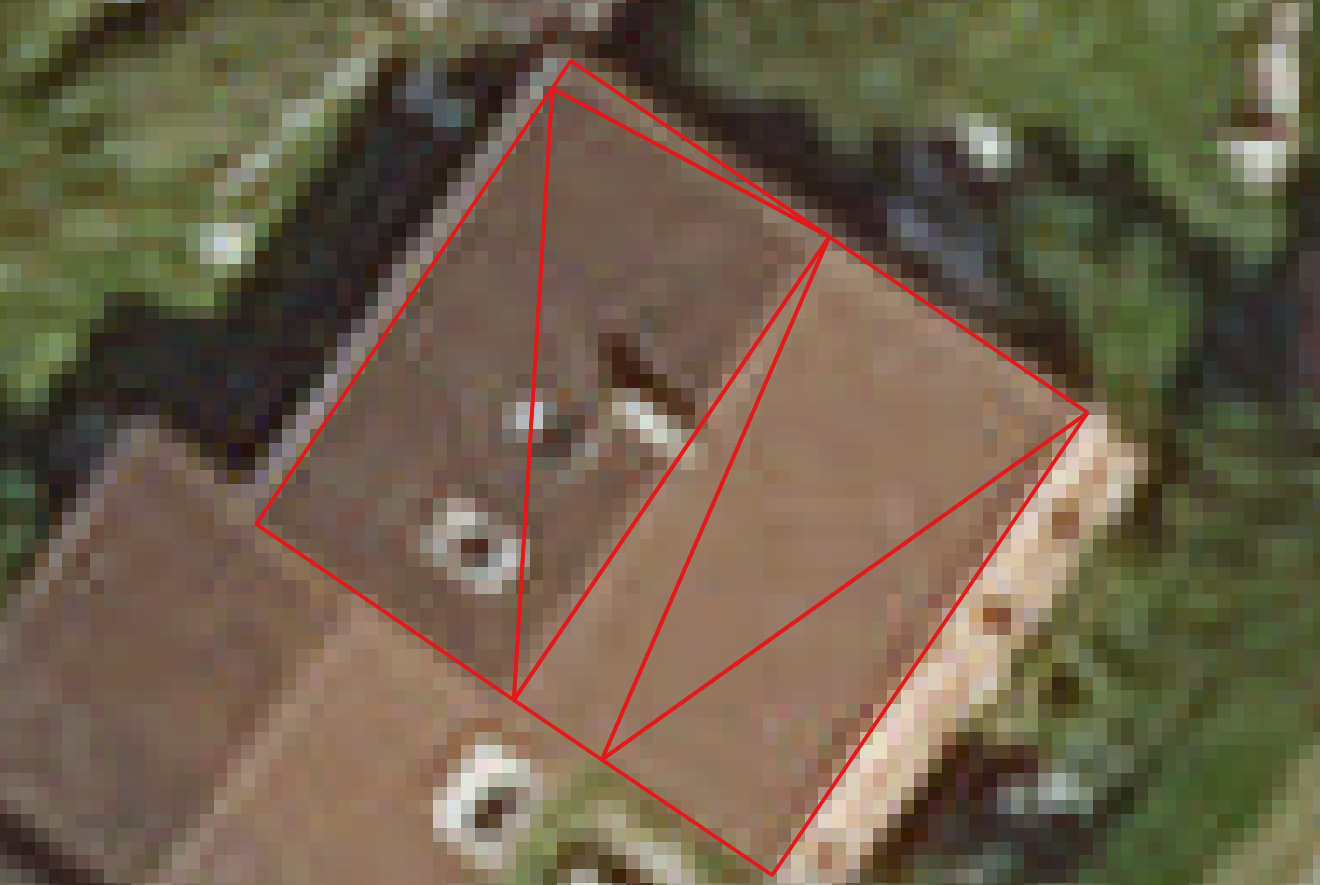
\includegraphics[width=\textwidth]{images/errors/facet/over_segmentation}}
                                \caption{\label{fig::fac_over} Facet over segmentation}
                            \end{subfigure}
                            \hspace{10pt}
                            \begin{subfigure}{.28\textwidth}
                                \fbox{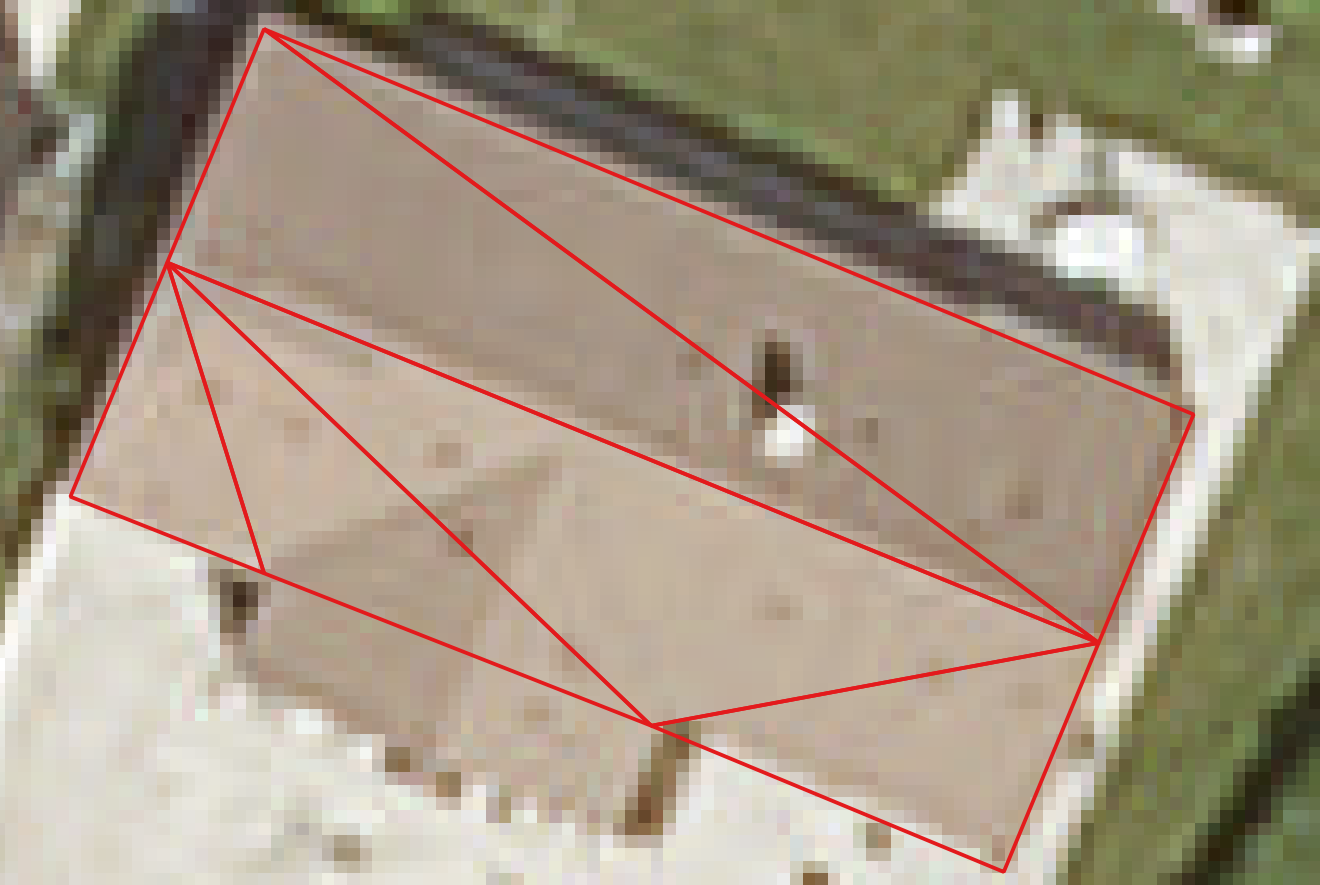
\includegraphics[width=\textwidth]{images/errors/facet/mis_segmentation}}
                                \caption{\label{fig::fac_footprint} Facet imprecise borders}
                            \end{subfigure}
                            \hspace{10pt}
                            \begin{subfigure}{.28\textwidth}
                                \fbox{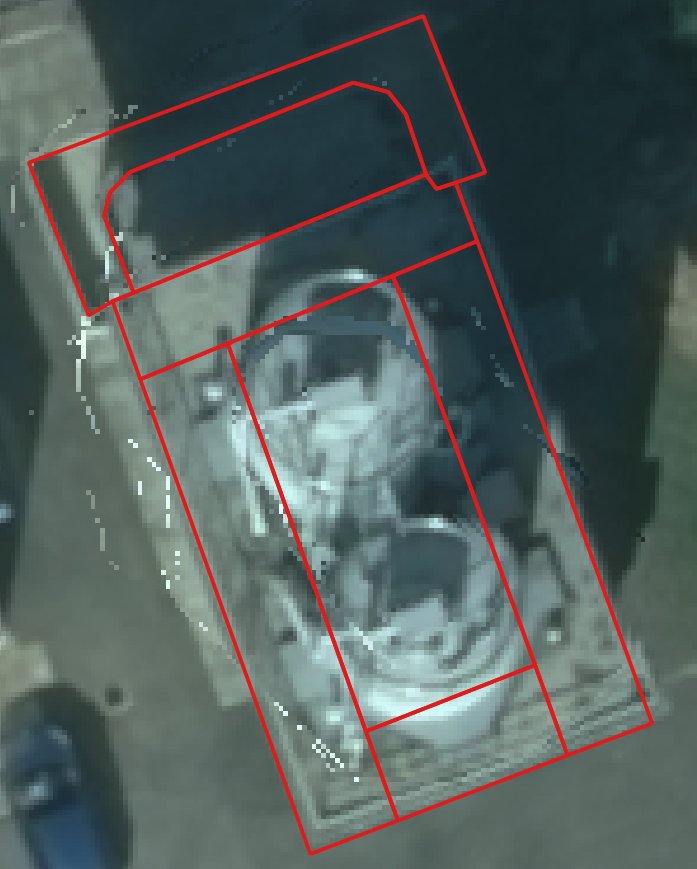
\includegraphics[width=\textwidth]{images/errors/facet/topology}}
                                \caption{\label{fig::fac_height} Inaccurate topology}
                            \end{subfigure}
                            \hspace{10pt}
                            \begin{subfigure}{.28\textwidth}
                                \fbox{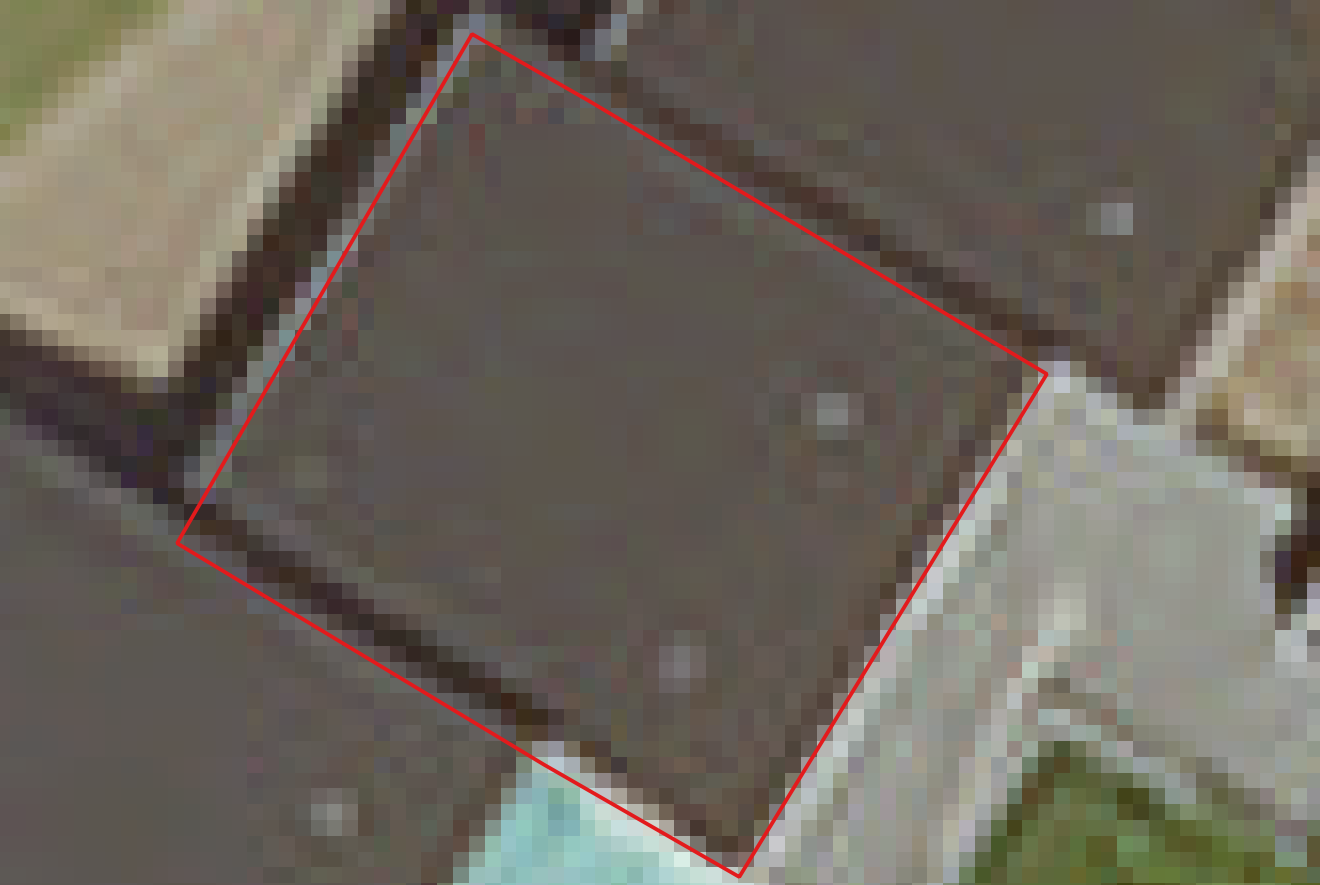
\includegraphics[width=\textwidth]{images/errors/facet/slope}}
                                \caption{\label{fig::fac_height} Imprecise geometry}
                            \end{subfigure}
                            \caption{Facet \emph{atomic} errors illustration.}
                        \end{center}
                    \end{figure}
                }
            \end{frame}
            \begin{frame}{Taxonomy parameters}
                The qualification has $3$ parameters:
                \begin{itemize}[label=$\blacktriangleright$, font=\color{IGNGreen}]
                    \item<1-> \emph{finesse}: the semantic level desired;
                    \item<2-> $\acrshort{acr::elod}$: the evaluation level of details;
                    \item<3-> \emph{exclusivity}: report only the lowest \acrshort{acr::lod}- errors (\emph{exclusive}) or all errors (\emph{non exclusive}).
                \end{itemize}
            \end{frame}
            \begin{frame}{Error taxonomy summary}
                \begin{figure}
                    \includestandalone[mode=buildnew, width=\textwidth]{taxonomy_tree}
                \end{figure}
            \end{frame}
        \subsection{Extracted features}
        \subsection{Classification process}
            \begin{frame}{Classifier}
                We opted for a \textbf{Random Forest} classifier, because:
                \begin{itemize}[label=$\blacktriangleright$, font=\color{IGNGreen}]
                    \item<1-> it handles well multimodal features;
                    \item<2-> being based on a boosting method, it is build to avoid overfitting;
                    \item<3-> it computes quite easily feature importance.
                \end{itemize}
                \uncover<4->{
                    Used parameters:
                    \begin{itemize}[label=$\blacktriangleright$, font=\color{IGNGreen}]
                        \item<5-> $4$ maximum depth to avoid overfitting the trees;
                        \item<6-> $1000$ trees to cover the whole the attributes space.
                    \end{itemize}
                }
            \end{frame}
            \begin{frame}{Classification problems summary}
                \begin{table}
                    \tiny
                    \begin{center}
                        \begin{tabular}{x{.05\textwidth} x{.06\textwidth} x{.05\textwidth} x{.7\textwidth}}
                            \toprule
                            \rotatebox{90}{\textbf{\textit{finesse}}} & \rotatebox{90}{\textbf{\acrshort{acr::elod}}} & \rotatebox{90}{\textbf{exclusivity}} & \textbf{Classification output}\\
                            \midrule
                            \scriptsize
                            \textcolor{green}{$1$} & -- & -- & Binary(Valid, Erroneous)\\
                            \textcolor{purple}{$2$} & \acrshort{acr::lod}-$1$ & -- & Binary(Valid, Building error)\\
                            \textcolor{purple}{$2$} & \acrshort{acr::lod}-$2$ & \textcolor{IGNDarkGreen}{on} & MultiClass(Valid, Building error, Facet error)\\
                            \textcolor{purple}{$2$} & \acrshort{acr::lod}-$2$ & \textcolor{red}{off} & MultiLabel(Valid, Building error, Facet error)\\
                            \textcolor{blue}{$3$} & \acrshort{acr::lod}-$1$ & \textcolor{IGNDarkGreen}{on} & MultiLabel(children(Binary(Valid, Building error)))\\
                            \textcolor{blue}{$3$} & \acrshort{acr::lod}-$2$ & \textcolor{IGNDarkGreen}{on} & MultiLabel(children(MultiClass(Valid, Building error, Facet error)))\\
                            \textcolor{blue}{$3$} & \acrshort{acr::lod}-$1$ & \textcolor{red}{off} & MultiLabel(children(Building error))\\
                            \textcolor{blue}{$3$} & \acrshort{acr::lod}-$2$ & \textcolor{red}{off} & MultiLabel(children(Building error)$\cup$ children(Facet error))\\
                            \bottomrule
                        \end{tabular}
                    \end{center}
                \end{table}
            \end{frame}

    \section{Experiments}
        \subsection{Used data}
        \subsection{Results}
        \subsection{Discussion}
            \begin{frame}{Some failure cases}
                \begin{figure}
                    \begin{center}
                    \tiny
                        \begin{tabular}{| x{.06\textwidth} | x{.035\textwidth} | x{.035\textwidth} || x{.06\textwidth} | x{.035\textwidth} | x{.035\textwidth} || x{.06\textwidth} | x{.035\textwidth} | x{.035\textwidth} || x{.06\textwidth} | x{.035\textwidth} | x{.035\textwidth} |}
                            \hline
                            \multicolumn{3}{| c ||}{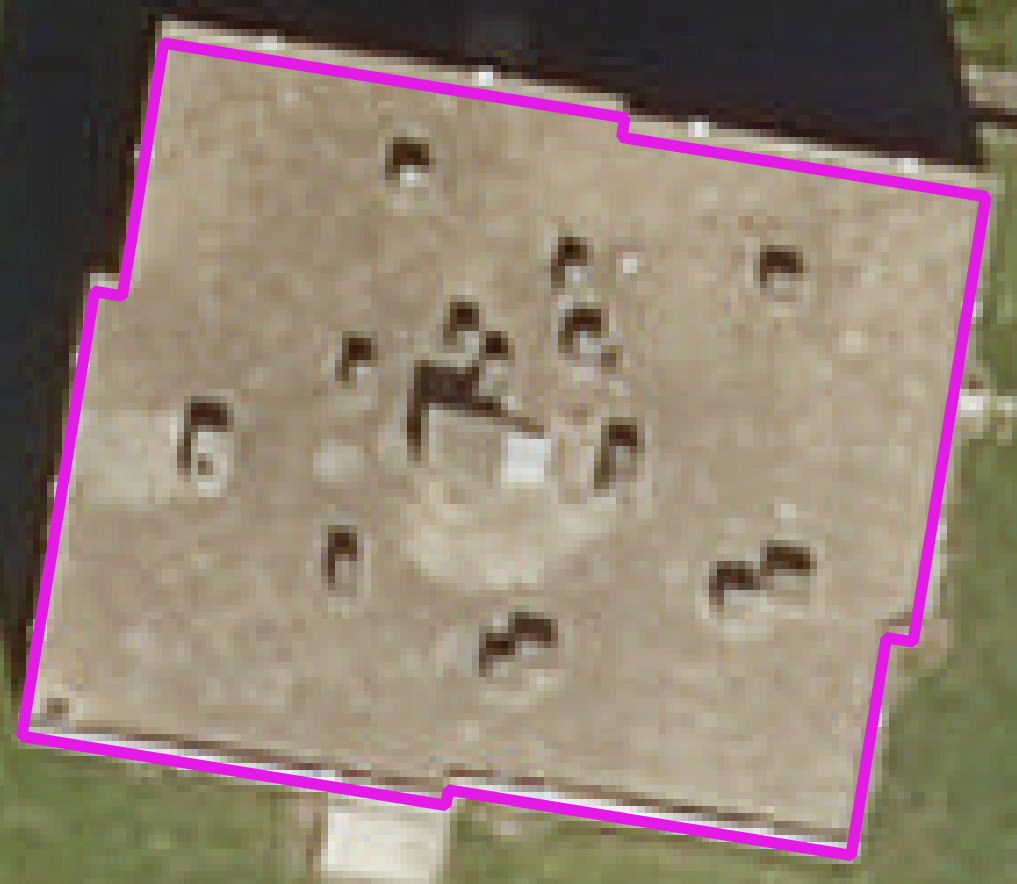
\includegraphics[width=.2\textwidth,valign=m,margin=1pt 1pt]{images/prediction_results/valid_as_bul_over}} & \multicolumn{3}{ c ||}{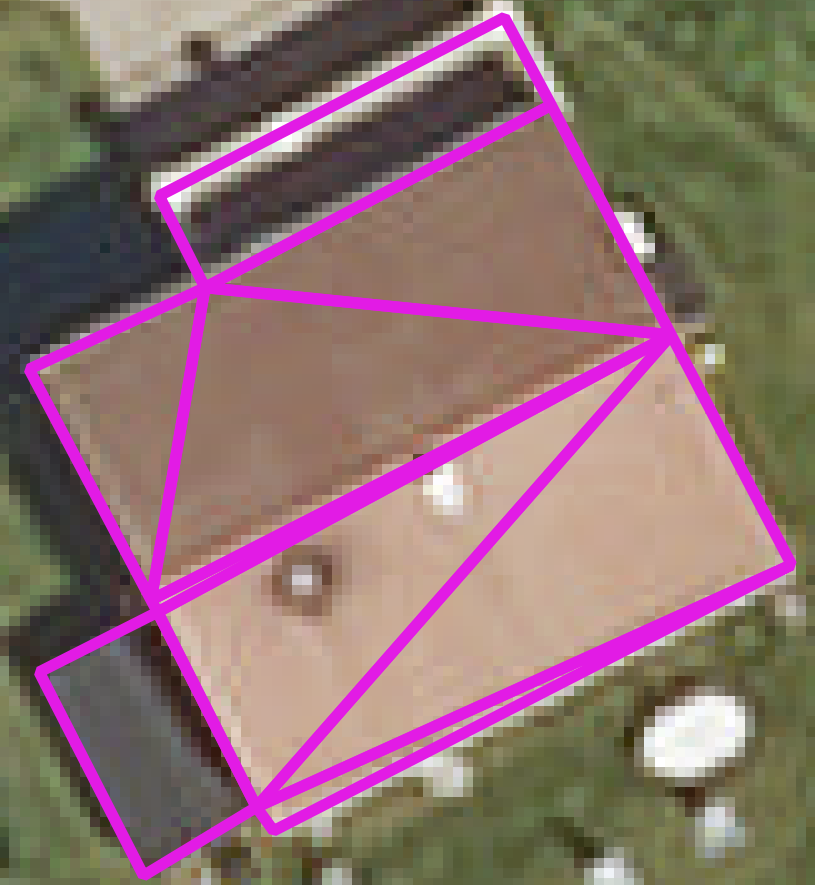
\includegraphics[width=.2\textwidth,valign=m,margin=0cm 1pt]{images/prediction_results/no_imprec_no_fac_over}} & \multicolumn{3}{ c ||}{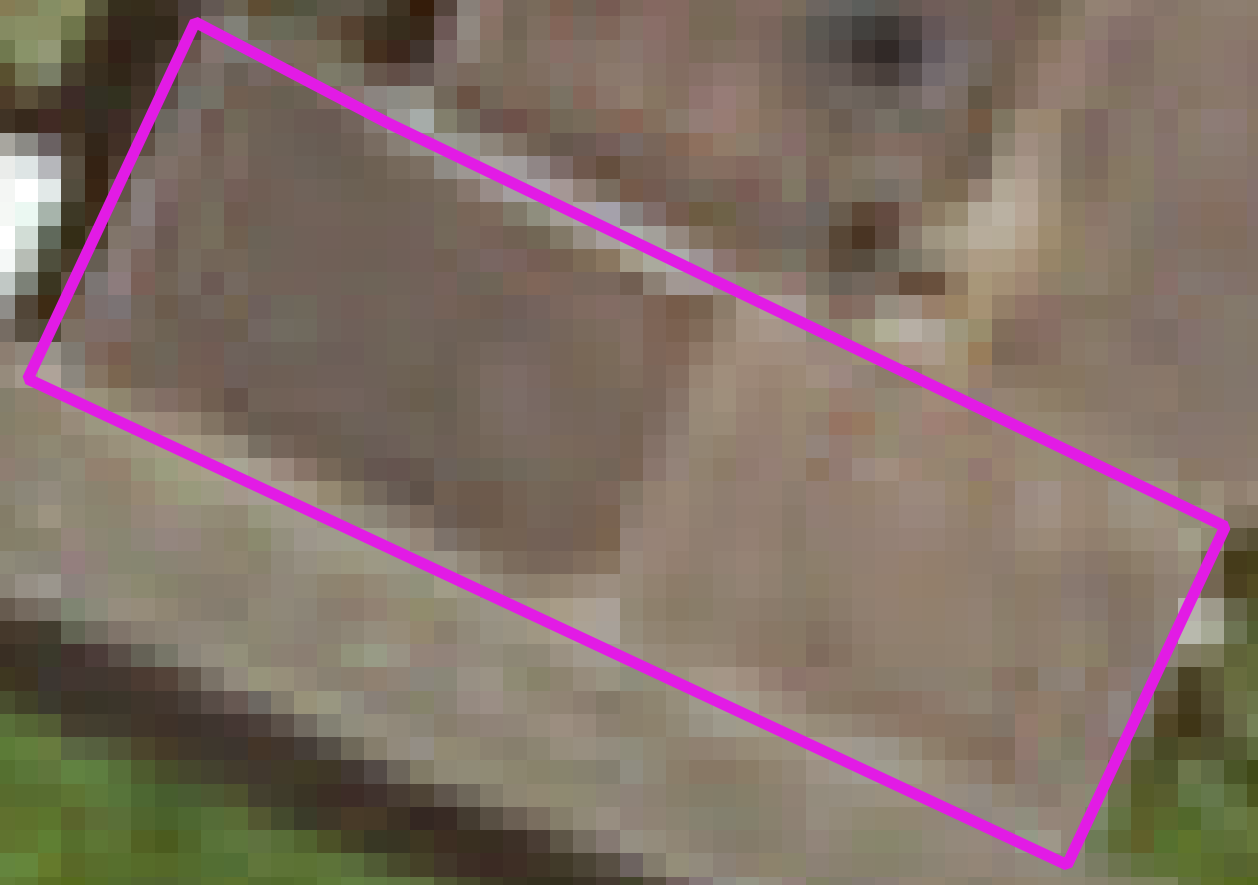
\includegraphics[width=.2\textwidth,valign=m,margin=0cm 1pt]{images/prediction_results/no_under_seg}} & \multicolumn{3}{ c |}{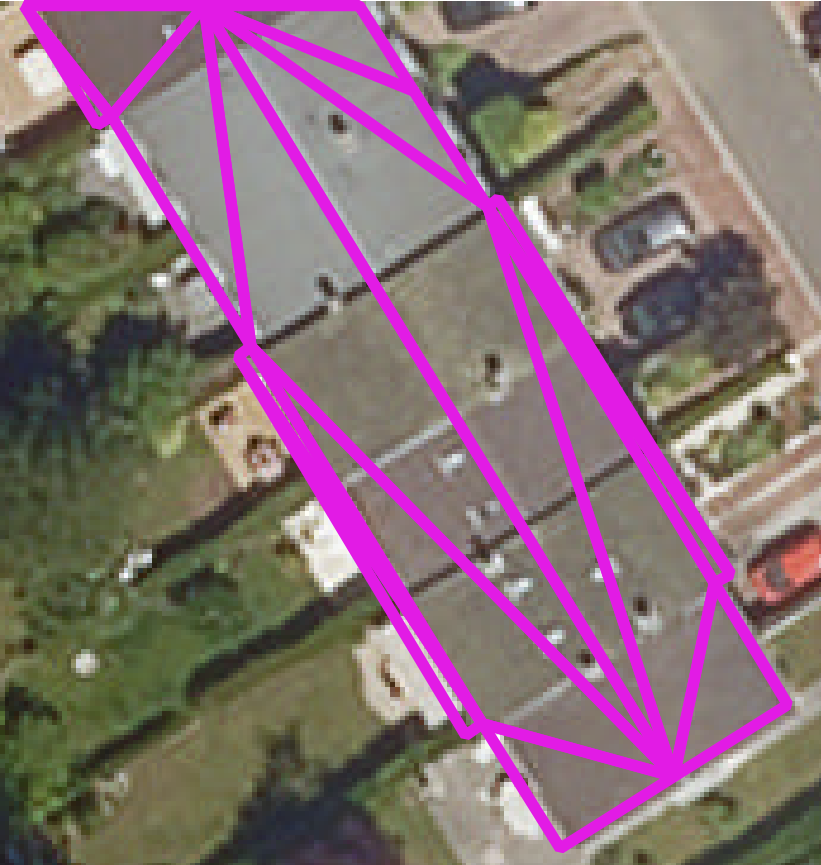
\includegraphics[width=.2\textwidth,valign=m,margin=0cm 1pt]{images/prediction_results/no_bul_under_seg}} \\
                            \hline
                            \textbf{Errors} & \textbf{G.T.} & \textbf{Pred.} & \textbf{Errors} & \textbf{G.T.} & \textbf{Pred.} & \textbf{Errors} & \textbf{G.T.} & \textbf{Pred.} & \textbf{Errors} & \textbf{G.T.} & \textbf{Pred.}\\
                            \hline
                            \textit{BOS} & \xmark & \cmark & \textit{BUS} & \xmark & \cmark & \textit{BOS} & \cmark & \cmark & \textit{BOS} & \cmark & \xmark \\
                            Valid & \cmark & \xmark & \textit{FImS} & \cmark & \xmark & \textit{FUS} & \cmark & \xmark &  \textit{FOS} & \cmark & \xmark \\
                             &  &  & \textit{FOS} & \cmark & \xmark &  &  &  & \textit{BUS} & \cmark & \xmark \\
                             &  &  &  &  &  &  &  &  &  \textit{BInF} & \cmark & \cmark \\
                            \hline
                        \end{tabular}
                    \end{center}
                \end{figure}                
            \end{frame}
    
    \section{Conclusion}
        \subsection{Percpectives}
            \begin{frame}{More annotated data}
                
            \end{frame}
            \begin{frame}{More sophisticated features}
                
            \end{frame}
        \subsection{Take home message}
            \begin{frame}{Take home message}
                
            \end{frame}
\end{document}